\section{Area-source proxy construction}
\label{sec:area-source-proxies}

\subsection{From residual mass to within-cell weights}

After point-source matching, the remaining proxy problem concerns
emissions that are represented by CAMS as area sources. These emissions
do not have a unique facility coordinate. They must therefore be
distributed inside each CAMS cell using spatial information that is
consistent with the activity represented by the sector. The role of an
area-source proxy is to provide this intra-cell distribution while
preserving the CAMS mass in the parent cell.

The area-source workflow follows the conservation principle introduced
in Section~\ref{sec:framework}. For each sector, one or more spatial
indicators are prepared on the common fine grid. These indicators are
converted into a non-negative raw score and then normalised within each
CAMS cell. The proxy therefore changes only the spatial distribution
inside the coarse cell; it does not revise the sectoral or pollutant
total reported by the inventory.

The difficulty is that the appropriate spatial evidence is sector
dependent. Shipping requires marine-traffic and port information. The
residual area component of public power follows a different logic,
because most large emissions are already handled as point sources and
the remaining CAMS area mass represents an inventory residual. Other
sectors require combinations of land use, infrastructure, population,
reported activity, or process-specific drivers. The following area-source
sections are therefore organised by methodological complexity rather than
by GNFR order.

\begin{figure}[htbp]
  \centering
  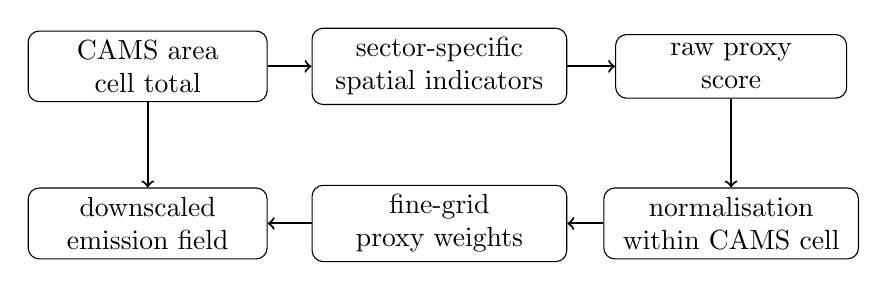
\begin{tikzpicture}[x=0.95cm,y=0.95cm]
    \node[draw, rounded corners, align=center, text width=2.8cm] (cams) at (0,0)
      {CAMS area\\cell total};
    \node[draw, rounded corners, align=center, text width=3.0cm] (drivers) at (3.9,0)
      {sector-specific\\spatial indicators};
    \node[draw, rounded corners, align=center, text width=2.7cm] (score) at (7.8,0)
      {raw proxy\\score};
    \node[draw, rounded corners, align=center, text width=3.0cm] (norm) at (7.8,-2.1)
      {normalisation\\within CAMS cell};
    \node[draw, rounded corners, align=center, text width=3.0cm] (weights) at (3.9,-2.1)
      {fine-grid\\proxy weights};
    \node[draw, rounded corners, align=center, text width=2.8cm] (mass) at (0,-2.1)
      {downscaled\\emission field};

    \draw[->, line width=0.75pt] (cams) -- (drivers);
    \draw[->, line width=0.75pt] (drivers) -- (score);
    \draw[->, line width=0.75pt] (score) -- (norm);
    \draw[->, line width=0.75pt] (norm) -- (weights);
    \draw[->, line width=0.75pt] (weights) -- (mass);
    \draw[->, line width=0.75pt] (cams) -- (mass);
  \end{tikzpicture}
  \caption{General area-source proxy workflow. Sector-specific spatial indicators define a raw score, which is normalised within each CAMS cell before being used to redistribute the corresponding CAMS area-source mass.}
  \label{fig:area-source-workflow}
\end{figure}

\begin{table}[htbp]
  \centering
  \caption{Area-source proxy families used in the upgraded workflow.}
  \label{tab:area-source-families}
  \begin{tabular}{p{0.22\textwidth} p{0.32\textwidth} p{0.22\textwidth} p{0.14\textwidth}}
    \toprule
    Proxy family & When it is used & Examples & Output type \\
    \midrule
    Generic proxy & A small number of robust indicators is sufficient, or the CAMS area mass is a residual component & Shipping; residual public power & Single area-weight layer \\
    Combined-dataset proxy & Several spatial drivers are needed to represent subsectors or activity groups & Waste; industry; fugitive emissions; off-road transport & Sector or pollutant-specific weight layers \\
    Highly customised proxy & The sector requires process-specific allocation or detailed subsector-to-driver mapping & Agriculture; solvents; other combustion & Pollutant or process-weighted layers \\
    \bottomrule
  \end{tabular}
\end{table}

\subsection{Generic area-source proxies}
\label{sec:generic-area-proxies}

Generic proxies are used where a simple spatial logic is scientifically
more defensible than an unnecessarily detailed construction. This does
not mean that the proxy is arbitrary. Rather, the sector either has a
dominant spatial driver that can be represented by a limited set of
harmonised datasets, or the area-source component is a residual mass for
which a complex process decomposition would not be meaningful. In the
current workflow, this category includes shipping and the residual
area-source component of public power. Aviation is kept as a future
generic-proxy candidate because it has not yet been implemented.

\subsubsection{Shipping}
\label{sec:generic-shipping}

Shipping is treated as a single area-source proxy shared by all
pollutants. This choice is appropriate because the main spatial question
is not pollutant-specific process disaggregation, but the recovery of a
plausible maritime and port-related support within the CAMS shipping
cells. The same vessel routes and port environments are relevant for the
allocation of the different shipping pollutants at the resolution used
here.

The proxy combines three spatial indicators. Vessel-density information
provides the main marine-traffic signal and identifies offshore shipping
corridors. Open mapping of port and harbour infrastructure refines the
coastal support. CORINE port-related land cover provides a harmonised
land-cover anchor for port areas. The raw proxy score is defined as a
weighted combination of these three components:

\begin{equation}
  S_{\mathrm{ship}} =
  0.25 D_{\mathrm{vessel}} +
  0.50 D_{\mathrm{port,osm}} +
  0.25 D_{\mathrm{port,clc}},
\end{equation}

where $D_{\mathrm{vessel}}$ is the scaled vessel-density field,
$D_{\mathrm{port,osm}}$ the scaled port-infrastructure support, and
$D_{\mathrm{port,clc}}$ the scaled CORINE port-area support. The larger
weight assigned to the mapped port-infrastructure term reflects its role
as the most explicit high-resolution coastal anchor, while the vessel
density term preserves the offshore traffic structure and the CORINE
term stabilises the port signal in a harmonised European land-cover
framework.

The resulting score is normalised within each CAMS shipping cell. The
final layer is therefore an allocation field rather than an emission
field: it determines how the CAMS shipping total is distributed inside
each parent cell, while preserving the original CAMS mass.

\begin{figure}[htbp]
  \centering
  \begin{subfigure}[b]{0.3\textwidth}
    \centering
    \includegraphics[width=\textwidth, height=4cm, keepaspectratio]{figures/Proxies/shipping_bbox_corine_port_area.png}
    \caption{CORINE port-area}
  \end{subfigure}
  \hfill
  \begin{subfigure}[b]{0.3\textwidth}
    \centering
    \includegraphics[width=\textwidth, height=4cm, keepaspectratio]{figures/Proxies/shipping_bbox_osm_port_area.png}
    \caption{OSM port infrastructure}
  \end{subfigure}
  \hfill
  \begin{subfigure}[b]{0.3\textwidth}
    \centering
    \includegraphics[width=\textwidth, height=4cm, keepaspectratio]{figures/Proxies/shipping_bbox_vessel_density.png}
    \caption{Vessel density}
  \end{subfigure}
  \caption{Visualization of the three spatial proxy components for shipping
    in the Athens area: (a) CORINE land cover (green), (b) OpenStreetMap
    port infrastructure (purple), and (c) vessel density (yellow).}
  \label{fig:athens-shipping-proxies}
\end{figure}

\subsubsection{Residual public power area emissions}
\label{sec:generic-public-power}

Public power is a mixed sector. The main combustion plants are handled
through point-source matching, because they correspond to discrete
facilities. The remaining CAMS area-source component has a different
interpretation. It is not treated as a separate set of known plants, but
as the residual mass left after the inventory reconciles national totals
with explicitly represented point sources. For this reason, a highly
detailed industrial proxy would give a false impression of process
specificity.

The residual area proxy follows the same broad logic used in the CAMS
allocation of unresolved public-power emissions: the residual total is
distributed using population as the main spatial gradient. The upgraded
proxy keeps this population-based logic for consistency with CAMS, but
amplifies the score where the fine grid contains eligible land cover.
Eligible land is defined as CORINE industrial or commercial land and the
equivalent harmonised industrial/built class used on the proxy reference
grid. These pixels are interpreted as more plausible locations for
residual energy-related activity than purely residential or natural
surfaces.

For each fine-grid pixel $j$ inside a CAMS area cell, let
$I_j^{\mathrm{elig}}$ be equal to one on eligible land and zero
elsewhere, and let $P_{01,j}$ be the population field scaled to the
range $[0,1]$ within the same CAMS cell. The raw proxy score is then

\begin{equation}
  S_{\mathrm{pp},j} =
  0.70 \left(I_j^{\mathrm{elig}}\right)^{1 + P_{01,j}}
  + 0.30 P_{01,j},
\end{equation}

where the first term gives priority to eligible land and the second term
retains the population-driven distribution used for the unresolved CAMS
component. This form keeps most of the support on eligible land while
still allowing population to redistribute residual emissions where the
land-cover signal is weak or incomplete.

\begin{figure}[htbp]
  \centering
  \begin{subfigure}[b]{0.3\textwidth}
    \centering
    \includegraphics[width=\textwidth, height=4cm, keepaspectratio]{figures/Proxies/publicpower_bbox_eligible_landcover.png}
    \caption{CORINE eligible land cover}
  \end{subfigure}
  \hfill
  \begin{subfigure}[b]{0.3\textwidth}
    \centering
    \includegraphics[width=\textwidth, height=4cm, keepaspectratio]{figures/Proxies/publicpower_bbox_population_proxy.png}
    \caption{Population proxy}
  \end{subfigure}
  \hfill
  \begin{subfigure}[b]{0.3\textwidth}
    \centering
    \includegraphics[width=\textwidth, height=4cm, keepaspectratio]{figures/Proxies/publicpower_bbox_weights.png}
    \caption{Weights}
  \end{subfigure}
  \caption{Visualization of the two spatial proxy components for PublicPower and the derived weights
    in the Athens area: (a) CORINE land cover (blue), (b) Population (red), and (c) weitghs. Blue lines correspond to CAMS cells }
\label{fig:athens-publicpower-proxies}
\end{figure}



If a CAMS cell contains no eligible land-cover support, the proxy falls
back to population weighting over the valid cell footprint. If population
also provides no usable support, a uniform distribution is used as a last
resort. These fallbacks preserve the CAMS area-source mass while making
the loss of spatial evidence explicit.

\subsubsection{Aviation}
\label{sec:generic-aviation}

Aviation is reserved as a future generic-proxy sector. It has not yet
been implemented in the upgraded workflow and is therefore not used in
the present downscaling chain. When implemented, it should be treated
with the same logic as the other area-source sectors: the proxy should
identify the appropriate airport and flight-activity support, normalise
the resulting score within CAMS cells, and preserve the CAMS sectoral
mass. Until that methodology is implemented and validated, no aviation
area-source proxy is reported here.
